\chapter{Implementation Approach}
\label{chap:implementation}
\lhead{\emph{Implementation Approach}}

\section{Architecture} \label{sec:Arch}
This application will have a HTML5, CSS3 and AngularJS front-end. Here is where the general look of our application will be done.
\begin{itemize}
    \item HTML5 provides the structure of the web application. Tags are used to describe the visual representation of the application, these are the building blocks of web pages. Tags are not displayed but they are used to render the content to the page. 
    \item CSS works in conjunction with HTML. It describes how the HTML elements are to be displayed on screen. This is particularly useful for viewing the application no different screen sizes. CSS allows for a dynamic and responsive web page. 
    \item AngularJS is a structural framework for dynamic web apps. It allows use of HTML as a template and enables the extension of HTML's syntax to express the application's components in a brief and clearly expressed manner.
\end{itemize}
This work will be done using Sublime Text 3 as this has lots of useful shortcuts that will reduce development time. 

The logic of the application will be done using a C Sharp back-end. Here is where our checks and general operations will be written. C Sharp is one of the most popular programming languages out there as it has many uses so this will come in useful when debugging and general fixes as there is a lot of documentation and helpful information out there. It's also useful for maintaining code as easily readable for programmers. This work will be done using Microsoft Visual Studio. 

The database chosen for this is Microsoft SQL Database. This being another Microsoft product, visual studio provides native support for programming with Microsoft SQL Database. Microsoft SQL Database can be used to visually observe and analyze queries and optimize the database performance. Tables can also be easily maintained and altered adding or removing columns where necessary. An important point to make about our database too is that passwords will not be stored, encryption will make this possible.

Unit and end too end tests will also be used to maintain code. These are often overlooked in projects but are absolutely vital. The logic will be tested by our unit tests, here we test that a function works as intended, end too end tests then test the UI of our application. Here we test things such as a button bringing you to the correct location. These tests are so important for large projects because when implementing new functionality it could unexpectedly impact old functions. These tests will be run using Jenkins continuous integration tool. This way we can automate the testing of our code and be notified of any defects immediately.

All source code will them be stored in internal GIT repositories. These repositories make having different environments possible, such as the development, QA and production environments. 

The application will be managed through JIRA. JIRA is an issue management platform that allows easy management of issues throughout their entire lifecycle. It is highly customizable, and can be tailored to fit any workflow. It will be used to manage and track development, and is useful for sticking to time frames. 

\section{Risk Assessment}
The application will be regularly tested by McAfees security team for threats so by the end of the project any security flaws should be mitigated. User data is the heart of the application and if not attended too properly could lead to some fatal problems. Having 1500+ users, all of whoms data will be on 12+ servers protecting their information and keeping it consistent is vital. Not keeping data consistent could lead to some users not being able to use any internal McAfee applications. To sign into an applications users passwords must be the same on all servers. This could lead to a potentially disastrous scenario. For instance imagine we go to change a users password and we manage to do it on 11 servers but the final one is down and we miss this server, now we have inconsistent data which cannot happen. This scenario will have to be handled with care, before doing any operations we will have to check the servers and their availability. That's one way to deal with this potentially catastrophic error but what happens if we check the server availability and they're all good but as we traverse through one goes down, well then we have the same problem. To deal with this scenario we will have to implement a three-way handshake when changing users data along with a revert option if all servers don't respond.  

\section{Methodology}
For the development of this application an agile approach will be taken. This is where the different development environments come in useful. Development can be done in the development environment while testing can be done in the QA environment simultaneously. These different environments allow the ability to easily change things as we progress. Requirements are realistically always going to change throughout a project and that's why the agile methodology is the best one to follow. 

The use of JIRA is also vital for this methodology. The QA team can report any defects or bugs they find and create a job on JIRA. The QA team can then see that their issues are being worked on and for how long. This is where spring planning comes into the frame. Here the product owner and development team go through the application backlog and prioritize issues, while also providing acceptance criteria for completion. This is a skill that is often overlooked in Computer Science, communication is key to absolutely everything so developers and product owners need to be able to converse so that the product owner knows what's being done and so the developer knows what is to be done. 


\section{Implementation Plan Schedule}
The development process will start in early January. This will include setting the project up on GitHub along with all the different environments it needs. During this time, heavy emphasis will be put on the structure of the project, this is very important as a good foundation is vital as it will make it easier to update and maintain in the long run. 

Come February the plan is to have general functionality working and for the development environment to be live. The point of having this environment is to test what has been implemented so far and get a feel for application and get a better understanding of how the application will work in the real world. 

By the middle of March our QA environment should be live. Here the McAfee quality assessment team will be testing the application for any bugs while also giving suggestions on changes this could range from something as simple visual changes or a complete flow change. 

April will be bug fixing and any minor tweaks that need to be done. Here we should be on the final stage of the project so it's all about fine tuning.

May the production environment will be live. This will be a fully functional application that will be getting real world use by many users. Therefore the QA and bug fixing stage is vital as the QA team may see problems where a developer may not.

\begin{figure}[ht]
  \centering
      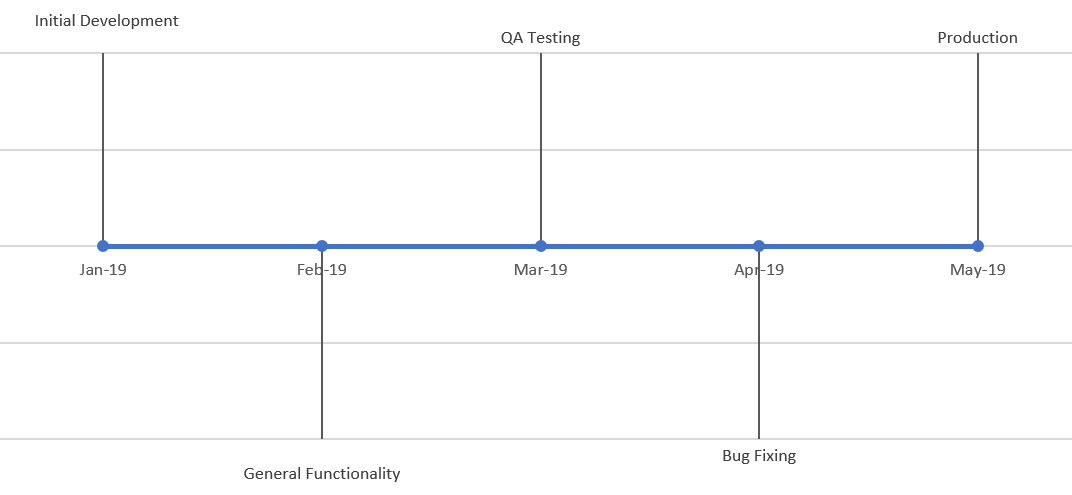
\includegraphics[width=1\textwidth]{MilestoneDiagram}
  \caption[Milestone Diagram]{Milestone Diagram}
  \label{fig:milestoneD}
\end{figure}

\section{Evaluation}
The number of bugs the project has will my main focus for the evaluation. If a project has even a lot of bugs, whether they are minor or major they make an application feel sloppy and unprofessional. Even something as simple as spelling mistakes or buttons getting misaligned when translating the application to another language can give a user a bad impression which could lead to loosing users.

Threat detection is another major part of the evaluation. This project will have thousands of users across multiple servers and their data must be kept secure. McAfees security team will be running regular checks on the application to make sure it is safe for all users. Threats can come from many areas of a projects, a simple one would be not checking input from a text box. All data entered by a user should be put through a black list check. The black list would contain things such as backslashes and double dots, these can be used by hackers to traverse the applications files and folders and potentially even run a cmd where anything would be possible from there. That's why threat detection and prevention is a vital focus.

The speed and responsiveness of the application is also another factor we must take into consideration. The applications code must be optimized to it's fullest. A sluggish application is unprofessional and cannot happen when it's being used for a business. The size of the project needs to be kept as low as possible as this will have a major impact on the load time, this can be done by making sure code is not duplicated or something as simple as making sure there are no unnecessary empty lines as these can increase file size. 

Readability of code is another important aspect to the project. This application will be used for potentially years and will be maintained and updated by numerous developers. Code should be easy to understand and well commented. 

\section{Prototype}
As stated previously a basic simplistic approach to the look of this project will be taken. This is necessary to give a intuitive nature to the application. our admin will be greeted to something like so. 
\begin{figure}[ht]
  \centering
      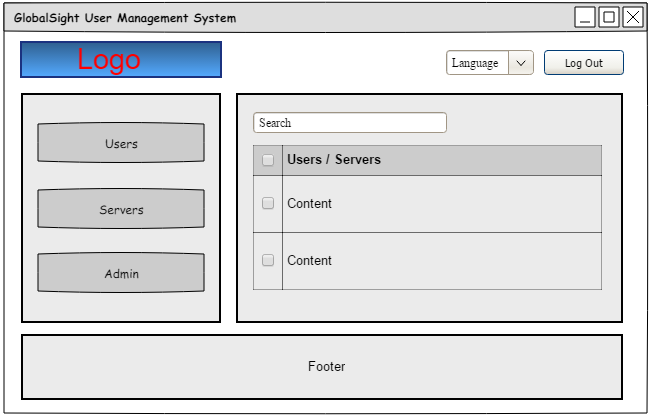
\includegraphics[width=1\textwidth]{Prototype1}
  \caption[Prototype 1]{Prototype 1}
  \label{fig:proto1}
\end{figure}

Our admin will be able to view our users and servers right away. Both will have the same table look with just different content. Our admin can then click on the desired user/Server where they can do their desired task such as reset password, set server groups etc. 

Upon clicking on an element such as a server our users will be greeted with a view like this. 
\begin{figure}[ht]
  \centering
      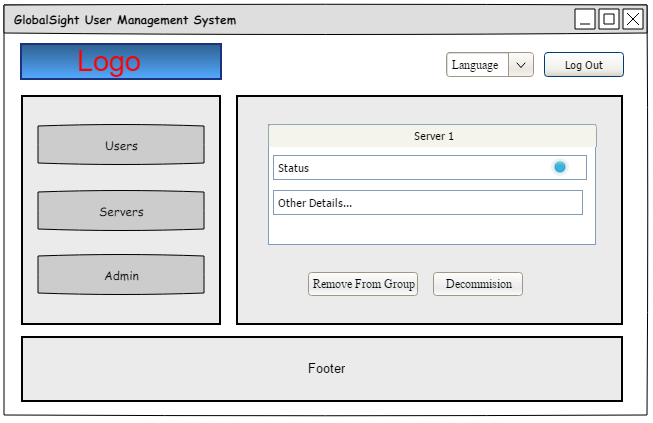
\includegraphics[width=1\textwidth]{Prototype2}
  \caption[Prototype 2]{Prototype 2}
  \label{fig:proto2}
\end{figure}

As you can see we plan on keeping the application looking more or less the same when traversing it again to give that intuitive feel. 